\chapter{Συμπεράσματα}
Το αποτέλεσμα της εκπόνησης της εργασίας είναι ένα πλήρης σύστημα διαχείρισης ραντεβού το οποίο μπορεί να διαμορφωθεί επαρκώς έτσι ώστε να καλύψει τις ανάγκες οποιασδήποτε επιχείρισης ανεξαρτήτου ειδικότητας και μεγέθους. Ο αρχικός σχεδιασμός αποδείχθηκε σωστός και έτσι το τελικό προϊόν λογισμικού πληροί τις απαιτήσεις για τις οποίες αναπτύχθηκε. 

\section{Προβλήματα}
Σε αυτήν την ενότητα περιγράφονται τα σημαντικότερα προβλήματα που αντιμετωπίστηκαν κατά την διάρκεια της ανάπτυξης του Easy!Appointments. Επεξηγούνται οι αποφάσεις που πάρθηκαν στην κάθε περίπτωση και αναλύονται οι λύσεις που χρησιμοποιήθηκαν.

\subsection{Διαχείριση χρόνου}
Σημαντικότερο πρόβλημα σχετικά με την υλοποίηση της εφαρμογής ήταν η χρονική καθυστέρηση μιας και ανάμεσα στην ανάληψη της εργασίας και την περαίωση της, πραγματοποιήθηκε η πρακτική άσκηση σε εταιρεία πληροφορικής καθώς και εργασία εκτός σχολής με άλλες εταιρείες του ίδιου τομέα. Οι εξωτερικές υποχρεώσεις αυτές αποσπούσαν την συνεχή και ομαλή ανάπτυξη, κάτι που συνεχώς διασπούσε τον ειρμό και τον δημιουργικό οίστρο. Συμπέρασμα αυτού του σημαντικού προβλήματος είναι ότι θα πρέπει να γίνεται σαφής και ορθός προγραμματισμός του χρόνου υλοποίησης ενός έργου γιατί διαφορετικά οι πιθανότητες για χαμηλότερη ποιότητα υπηρεσίας ή ακόμα και αποτυχίας του έργου αυξάνονται εκθετικά. Σε αυτό μπορεί να συντελέσει και η πληθώρα των εφαρμογών οι οποίες αποσκοπούν στην αποδοτικότερη διαχείριση έργων λογισμικού οι οποίες είναι διαθέσιμες είτε δωρεάν, είτε έναντι αμοιβής.

\subsection{Συγχρονισμός δεδομένων με το Google Calendar}
Όσον αφορά την συνεργασία του συστήματος με την υπηρεσία Google Calendar αλλά και γενικότερα με άλλες πιθανές υπηρεσίες το ζήτημα παραμένει στο πως θα παραμείνουν τα δεδομένα ακέραια και ενημερωμένα και στα δύο συστήματα, όταν δεν υπάρχει ένα κοινό μέσο αποθήκευσης. Το θέμα γιγαντώνεται μάλιστα όταν δεν υπάρχει πρόσβαση στον κώδικα του ενός από τα δύο συστήματα έτσι ώστε να δημιουργηθεί μια "γέφυρα δεδομένων". Για την επίλυση αυτού του θέματος ήταν αναγκαίο να δημιουργηθεί ένας αλγόριθμος συγχρονισμού ο οποίος θα ενεργοποιούνταν από την πλευρά του Easy!Appointments και θα αναλάμβανε την ενημέρωση και τον δύο συστημάτων με τα τελευταία δεδομένα. Για αυτόν τον σκοπό θα έπρεπε να καταγραφούν και να υλοποιηθούν κάποιοι κανόνες συγχρονισμού οι οποίοι θα μετέφεραν επιτυχώς τα ραντεβού αμφίδρομα και στα δύο συστήματα. Στις περιπτώσεις όπου η μεταφορά αυτή θα ήταν αδύνατη (σύγκρουση δεδομένων) ο χρήστης θα έπρεπε να αποφασίσει ποια εκδοχή των δεδομένων θα υπερισχύσει στο τέλος.

\subsection{Διαχωρισμός δικαιωμάτων χρηστών}
Ένα ακόμα πρόβλημα που αντιμετωπίστηκε κατά την διάρκεια την ανάπτυξης του έργου ήταν ο διαχωρισμός των δικαιωμάτων των χρηστών μέσα στο σύστημα. Ο κάθε χρήστης αναλόγως το είδος του (διαχειριστής, πάροχος, γραμματέας) έχει διαφορετικές δυνατότητες και δικαιώματα στα δεδομένα που αποθηκεύονται από το σύστημα. Αυτό συμβαίνει γιατί στις περισσότερες περιπτώσεις θα πρέπει να τηρηθεί η ιεραρχία της επιχείρησης αλλά και επίσης γιατί θα πρέπει να διασφαλιστεί η ακεραιότητα των δεδομένων από τυχόν εσφαλμένες ενέργειες χρηστών σε βασικές ρυθμίσεις του συστήματος. Για τις κυριότερες ρυθμίσεις απαιτούνται τα δικαιώματα διαχειριστή και έτσι το σύστημα χρειάζεται απαραιτήτως πάντα έναν χρήστη διαχειριστή (ο χρήστης που δημιουργείται κατά την εγκατάσταση είναι ουσιαστικά ο πρώτος διαχειριστής της εφαρμογής). Για να λυθεί αυτό το πρόβλημα η εγγραφή του κάθε χρήστη στην βάση δεδομένων συνδέεται με έναν ρόλο ο οποίος περιέχει τα δικαιώματα που του αντιστοιχούν. Έτσι για παράδειγμα ένας χρήστης που προορίζεται για πάροχος υπηρεσίας, θα έχει τα δικαιώματα που αντιστοιχούν στον ρόλο "Πάροχος Υπηρεσίας" όπως αυτά είναι αποθηκευμένα στην βάση δεδομένων. Έτσι κάθε φορά που συνδέεται ένας χρήστης στο διαχειριστικό κομμάτι της εφαρμογής τα δεδομένα σχετικά με τα δικαιώματα του και τον ρόλο του διαβάζονται από σελίδα σε σελίδα και η εφαρμογή μπορεί και γνωρίζει με ποιόν τρόπο θα πρέπει να εμφανιστούν τα δεδομένα και ποιες ενέργειες είναι διαθέσιμες στην κάθε περίπτωση.

\section{Εξέλιξη της εφαρμογής}
Όπως και σε κάθε έργο λογισμικού, υπάρχουν πολλά πράγματα τα οποία μπορούν να εξελιχθούν και να βελτιωθούν καθώς και δυνατότητες οι οποίες μπορούν να προστεθούν για να κάνουν την εφαρμογή πιο εύχρηστη και αποδοτικότερη. Οι βελτιώσεις αυτές γίνονται στην φάση της συντήρησης και επέκτασης σταδιακά, με σκοπό την ύπαρξη ενός ενημερωμένου προϊόντος στην αγορά. Με αυτόν τον τρόπο οι εταιρείες θα μπορούν να εμπιστεύονται την εν λόγω εφαρμογή και να την χρησιμοποιούν ως το δικό τους εργαλείο διαχείρισης των ραντεβού. Παρακάτω περιγράφονται κάποια σημεία στα οποία θα μπορούσε να εξελιχθεί μελλοντικά το σύστημα που παράχθηκε.

\subsection{Mobile design}
Με την πάροδο του χρόνου όλο και περισσότερες "έξυπνες" συσκευές βρίσκονται στα χέρια των καταναλωτών και έτσι δημιουργείται η ανάγκη για χρήση των διαδικτυακών εφαρμογών από οθόνες που έχουν διαφορετικά μεγέθη οθονών. Εφόσον η σχεδίαση για όλες τις διαστάσεις οθονών υπολογιστή έχουν καλυφθεί, το επόμενο βήμα είναι να σχεδιαστεί το σύστημα για κινητές συσκευές και tablet. Με αυτόν τον τρόπο θα μπορούν οι χρήστες του Easy!Appointments να χρησιμοποιούν το σύστημα από το κινητό τους πολύ πιο άνετα και έτσι να είναι πάντα ενημερωμένοι σχετικά με τα ραντεβού τους όπου και αν βρίσκονται. Προϋπόθεση για αυτό πάντα είναι μια ενεργή σύνδεση με το διαδίκτυο. Για να υλοποιηθεί αυτή η δυνατότητα θα χρειαστεί να γραφεί CSS κώδικας ο οποίος να εμφανίζει την εφαρμογή διαφορετικά σε κινητές συσκευές.

\subsection{Μετάφραση της διεπαφής χρήστη}
Η πρώτη υλοποίηση του συστήματος έχει γίνει εξολοκλήρου στην αγγλική γλώσσα όπως και με τα περισσότερα συστήματα που απευθύνονται σε ένα ευρύ καταναλωτικό κοινό. Το Easy!Appointments δέχεται κείμενο και σε άλλες γλώσσες (χρησιμοποιείται το encoding UTF-8) αλλά η διεπαφή, τα μηνύματα και τα αντικείμενα ελέγχου είναι όλα στα Αγγλικά. Για να γίνει πιο εύκολη η χρήση της εφαρμογής και από ανθρώπους οι οποίοι δεν είναι τόσο εξοικειωμένοι με αυτήν την γλώσσα θα πρέπει να μεταφραστεί όλο το σύστημα και σε άλλες κοινές γλώσσες. Για να επιτευχθεί αυτό στην συγκεκριμένη περίπτωση θα πρέπει να χρησιμοποιηθεί μια συγκεκριμένη τεχνική, όπως ενδεικνύεται από τον ιστότοπο του κατασκευαστή του CodeIgniter.

\subsection{Αναφορές δεδομένων}
Το σύστημα μέσω της λειτουργίας του κρατάει διάφορα δεδομένα (ραντεβού, πελάτες, πάροχοι κτλ). Καλό θα ήταν αυτά τα δεδομένα να μπορούν να εξαχθούν με κάποιον τρόπο έτσι ώστε να μπορέσουν να χρησιμοποιηθούν και με άλλους τρόπους. Μια περίπτωση χρήσης θα ήταν η εξαγωγή των σημερινών ραντεβού ενός πάροχου σε μια εκτυπώσιμη αναφορά έτσι ώστε να μπορεί ο χρήστης να την τυπώσει και να την έχει ως λίστα στο γραφείο. Μια άλλη περίπτωση χρήσης θα ήταν να εκτυπωθούν τα στοιχεία ενός πελάτη καθώς και το ιστορικό των ραντεβού του. Οι αναφορές αυτές είναι πολύ χρήσιμες γιατί μπορούν να αναδείξουν γρήγορα δεδομένα και μάλιστα σε εκτυπώσιμη μορφή, κάτι που χρειάζονται ακόμα πολλές εταιρείες.

\subsection{Στατιστικές πληροφορίες} 
Μια χρήσιμη μελλοντική δυνατότητα θα ήταν η συλλογή στατιστικών πληροφοριών σχετικά με τα ραντεβού που κλίνονται στο σύστημα. Από αυτήν την διαδικασία θα μπορούσαν να βγουν σημαντικές πληροφορίες όπως το ποια υπηρεσία ή πάροχος προτιμάται πιο συχνά, ποιες μέρες έχουν τα περισσότερα ραντεβού, πόσο συχνά ακυρώνονται τα ραντεβού και σε πόσο χρονικό διάστημα πριν. Αυτές οι πληροφορίες είναι πολύ σημαντικές για μια εταιρεία η οποία λειτουργεί με κρατήσεις ραντεβού γιατί έτσι μπορεί να γνωρίζει με ποιόν τρόπο λειτουργεί το πελατειακό κοινό της και έτσι να λειτουργεί αναλόγως για να παρέχει καλύτερη εξυπηρέτηση. Ένα παράδειγμα θα ήταν η περίπτωση ενός μεγάλου κομμωτηρίου στην οποία οι πελάτες θα κρατούσαν πάρα πολλά ραντεβού το Σάββατο κάθε εβδομάδας, γιατί πιθανόν έχουν περισσότερο χρόνο. Τα στατιστικά (εκτός της πείρας) θα έδειχναν την αυξημένη κίνηση του Σαββάτου και έτσι ο διαχειριστής θα είχε διαθέσιμους όλους του πάροχους προς ραντεβού, για να μπορέσει να καλυφθεί το κοινό όσο καλύτερα γίνεται.

\subsection{Δημιουργία RESTful υπηρεσίας}
Κάθε μεγάλο διαδικτυακό σύστημα παρέχει και μια RESTful υπηρεσία η οποία μπορεί να απαντάει με δεδομένα σε διάφορες κλήσεις που της γίνονται, εφόσον βέβαια έχει πιστοποιηθεί ο client που επικοινωνεί μαζί τους. Με αυτόν τον τρόπο θα μπορούν άλλοι προγραμματιστές να φτιάχνουν εφαρμογές οι οποίες θα επικοινωνούν με το Easy!Appointments και θα διαχειρίζονται τα δεδομένα του συστήματος. Η υλοποίηση αυτής της δυνατότητας θα βοηθούσε πολύ την εξέλιξη και την χρήση του Easy!Appointments γιατί από εδώ και πέρα διάφορες εφαρμογές θα υλοποιούνταν κάνοντας δυνατή την χρήση των δεδομένων σε πολλές διαφορετικές περιστάσεις. Κάτι που είναι πάρα πολύ χρήσιμο για κάθε επαγγελματία (παραδείγματος χάρη η χρήση πελατών από CRM εφαρμογή).

\subsection{Βελτίωση κώδικα}
Τελευταίο αλλά και όχι λιγότερο σημαντικό είναι η συνεχής βελτίωση και ενημέρωση του κώδικα έτσι ώστε να είναι πάντα στην καλύτερη δυνατή κατάσταση. Καθώς εξελίσσεται ένα σύστημα λογισμικού είναι απαραίτητο να βελτιώνεται ο κώδικας και η δομή του. Επίσης είναι απαραίτητο να ενημερώνονται και τα εξωτερικά εργαλεία τα οποία χρησιμοποιούνται έτσι ώστε να διασφαλίζεται η ασφάλεια και η ποιότητα του συστήματος. Κατά καιρούς εμφανίζονται διάφορες ενημερώσεις ασφαλείας αλλά και διορθώσεων σφαλμάτων σε αυτά τα framework (CodeIgniter, jQuery κτλ) τα οποία θα χρειαστεί να συμπεριληφθούν και στο Easy!Appointments. Κάθε φορά που ο χρήστης λαμβάνει μια νέα έκδοση της εφαρμογής θα πρέπει ο κώδικας που την απαρτίζει να βρίσκεται σε πολύ καλή κατάσταση, να έχει ελεγχθεί και να λειτουργεί σωστά έτσι ώστε να εμπνέει εμπιστοσύνη προς τους χρήστες.

\section{Πληροφορίες}
Η διαχείριση του έργου έγινε στην υπηρεσία Google Code και ο κώδικας είναι διαθέσιμος στην διεύθυνση \url{https://code.google.com/p/easy-appointments/}. Υπάρχει επίσης και η επίσημη ιστοσελίδα του Easy!Appointments στην διεύθυνση \url{http://easyappointments.org}.
\newline
\begin{figure}[H]
\centering
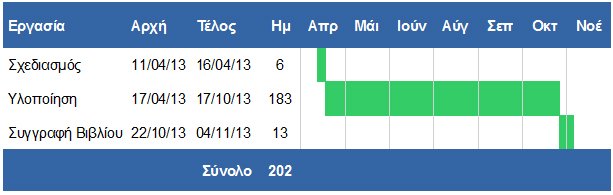
\includegraphics[width=150mm]{images/gantt-simple.jpg}
\caption{Χρονοδιάγραμμα Υλοποίησης (Gantt)}
\label{gantt-simple}
\end{figure}